\documentclass[11pt,twocolumn]{article}

\usepackage{graphicx}
\usepackage[iso]{datetime}
\usepackage{geometry}
\usepackage{titling}
\usepackage[default]{fontsetup}
\usepackage{kotex}
\usepackage{amsmath}
\usepackage{listings}
\usepackage{booktabs}
\usepackage[capitalise]{cleveref}
\usepackage[backend=biber,style=ieee,citestyle=ieee]{biblatex}

\addbibresource{src.bib}
\lstset{language=Matlab,numbers=left,breaklines=True,basicstyle=\footnotesize,upquote=true,showstringspaces=false,morekeywords={clearvars,struct,deal,optimoptions,fmincon,box,contourf,xlim,ylim}}
\geometry{a4paper,left=20mm,right=20mm,top=30mm,bottom=30mm}
% \setlength{\droptitle}{10mm}
\renewcommand*{\mkbibemph}[1]{\textsl{#1}}
\pretitle{\begin{center} \Huge}
\title{\textbf{Optimization of Total Operating Cost per Driving Range in Compact EVs}}
\posttitle{\par \vspace{5mm} \LARGE -Optimum Design Final Project- \par \end{center} \vspace{5mm}}

\preauthor{\begin{center} \large EME3031, Class 41, Group 1 \par \begin{tabular}[t]{c}}
\author{Kim Jaeju \thanks{2020310397, Solved, analyzed, and discussed about the problem with Excel.} \and Shin Taeha \thanks{2021314315, Solved, visualized, and discussed about the problem with \textsc{Matlab} and it. Edited the report.} \and Im Yebin \thanks{2024319449, Collected and organized data.} \and Jang Yongsun \thanks{2020310051, Defined and formalized the problem.}}
\postauthor{\vspace{1mm} \end{tabular} \par \normalsize School of Mechanical Engineering, Sungkyunkwan University \end{center}}

\date{\today}

\begin{document}
    \begin{titlepage}
        \maketitle
        \begin{abstract}
            In 2023, there were around 14 million EVs sold worldwide, accounting for almost 18\% of all new automobile purchases \cite{iea24}.
            In tandem with this expansion, battery pack costs decreased to roughly 139USD/kWh in 2023, a 90\% decrease since 2008, and additional drops are anticipated to reach 105USD/ kWh by 2025-2026 \cite{iea24}\cite{doe23}.
            This study uses body (glider) weight and battery capacity as essential factors to predict the overall operating cost per kilometer (KRW/km) of a compact electric vehicle.
            A consumer price ceiling, a minimum driving range, and a vehicle mass limit are some of the restrictions.
            In this study, we use both numerical (\textsc{Matlab} and Excel Solver) and graphical (analytical) optimization techniques.
            The findings pinpoint the ideal design point that minimizes cost per kilometer while satisfying range and pricing limits by balancing battery capacity and glider mass.
            The results provide useful advice for economical EV design in light of global decarbonization and consumer markets that are price conscious.
        \end{abstract}
    \end{titlepage}
    
    \begin{figure}[h]
        \centering
        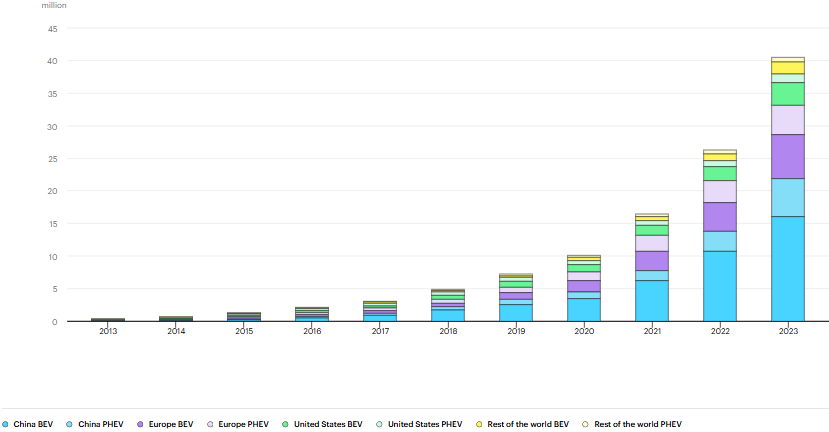
\includegraphics[width=0.8\columnwidth]{growth.png}
        \caption{Growth in Global EV stock.}
        \label{growth}
    \end{figure}

    \section{Introduction}
        \subsection{Motivation}
            See \cref{growth}.
            In 2023, almost 14 million electric vehicles (EVs) were sold worldwide, accounting for nearly 18\% of all new automobiles, and there were nearly 40 million EVs in total \cite{iea24}.
            Battery packs still account for 40-50\% of EV costs; therefore, despite this momentum, the initial cost of EVs remains a significant obstacle \cite{doe23}.
            Although battery prices have sharply declined, they are expected to drop much more by 2025, reaching approximately 105 USD/kWh. This could enable EVs to become as affordable as cars with internal combustion engines \cite{doe23}.
            Reducing the overall operational cost per mile, as opposed to just the purchase price, is crucial to accelerating adoption.
            \par
            Efficiency and operating costs are directly impacted by vehicle weight.
            Using materials or designs that minimize bulk can lower energy consumption by 6-8\% for every 10\% reduction in weight \cite{doe23b}.
            This could result in a longer range or a smaller battery.
            However, weight and purchase price increase when battery capacity increases.
            Therefore, there is a design trade-off: minimize per-kilometer costs by optimizing battery size and weight.
            \par
            South Korean politicians hope to have 4-4.5 million EVs on the road by 2030 with subsidies, but customers want reasonably priced cars with enough range.
            Even in urban settings, Korean drivers often choose larger models with longer driving ranges \cite{iea23}\cite{nrel23}.
            Consequently, calculating cost efficiency (KRW/km) under actual design restrictions is both academically and practically useful.
        \subsection{Objectives}
            The following are the goals we aim to achieve through this optimum design project.
                \begin{itemize}
                    \item Create a cost model that calculates the total operating cost, including energy expenses and battery depreciation.
                    \item Establish two design variables (DVs) to maintain an appropriate difficulty level and enable the use of various techniques.
                    \item Define realistic and reasonable constraints through thorough research.
                    \item To minimize the objective function, use optimization techniques: employ both analytical (graphical) and numerical (\textsc{Matlab}, Excel) approaches.
                    \item Examine the findings: identify the optimal point, perform analyses, and make suggestions for an economical EV design.
                \end{itemize}
        \subsection{Backgrounds}
            \subsubsection{Trend in the EV Batteries Market}
                As shown in \cref{batCost}, the cost of an EV battery pack decreased significantly from approximately 1,415 USD/kWh in 2008 to 139 USD/kWh in 2023.
                Due to ongoing advancements in battery technology and production efficiency, it is anticipated that costs will approach 105 USD/kWh by 2025-2026 \cite{doe23}\cite{nrel23}.
                \begin{figure}[h]
                    \centering
                    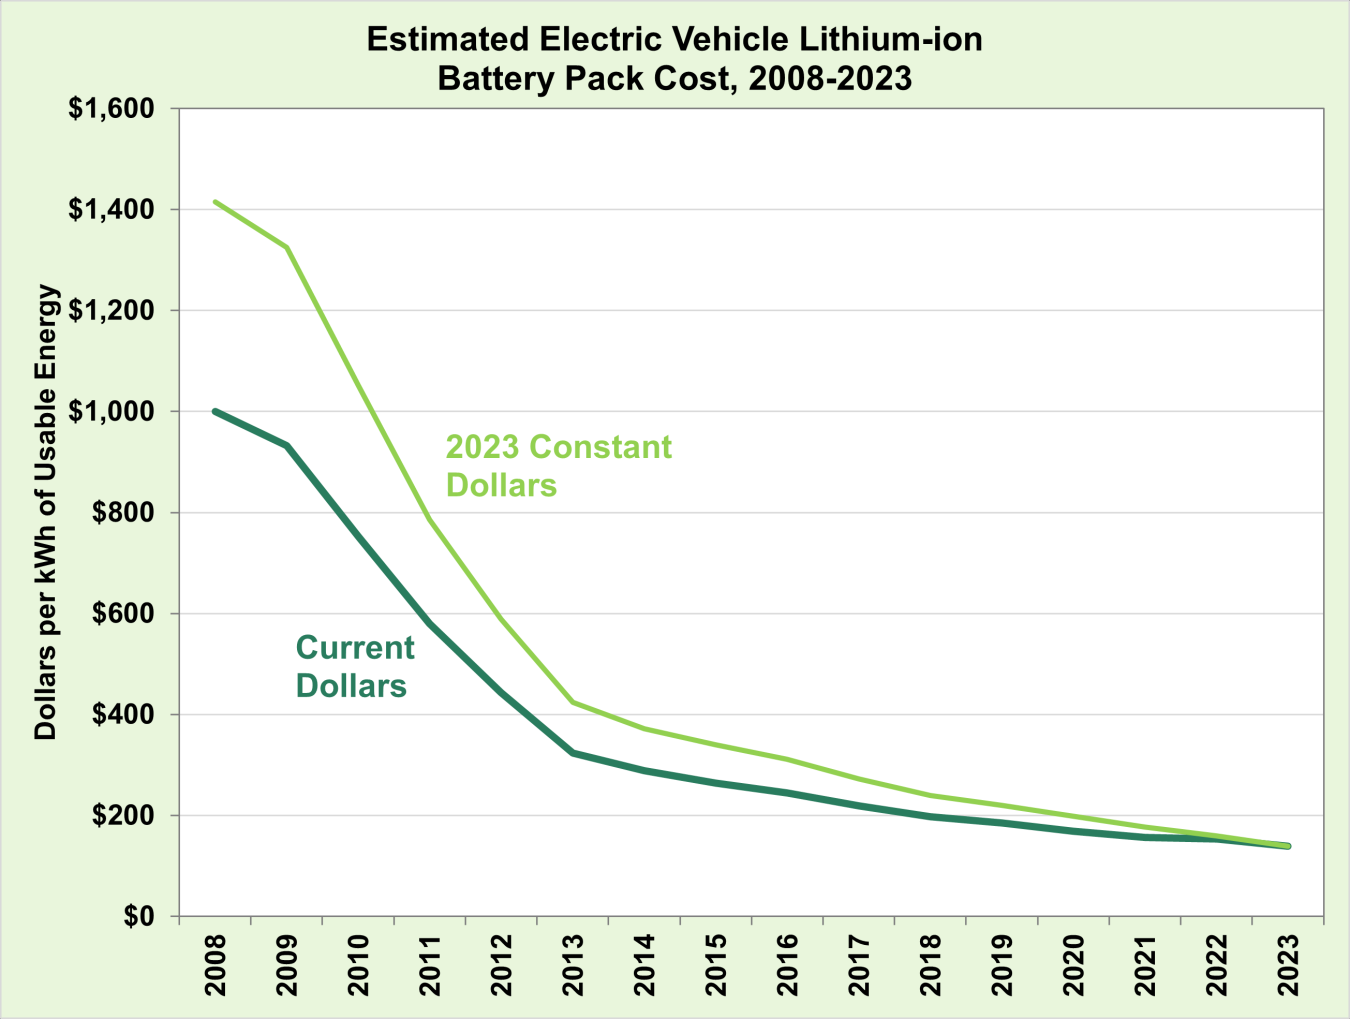
\includegraphics[width=.8\columnwidth]{batCost.png}
                    \caption{Declining EV Battery Prices.}
                    \label{batCost}
                \end{figure}

            \subsubsection{The Value of Being Lightweight}
                Reducing vehicle bulk directly increases efficiency.
                A 10\% decrease in vehicle weight typically leads to a 6-8\% boost in fuel efficiency \cite{doe23b}.
                Lighter cars use less energy per kilometer and can have smaller batteries while maintaining range.
                Studies show that reducing weight can balance out battery mass, improving range or lowering costs as you can see in \cref{gliderReduction} \cite{doe23b}\cite{nrel23}.

                \begin{figure}[h]
                    \centering
                    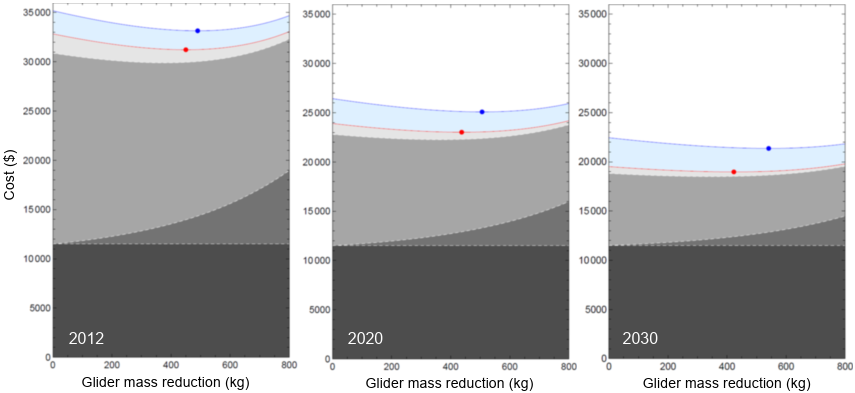
\includegraphics[width=.8\columnwidth]{gliderReduction.png}
                    \caption{Cost Based on Glider Weight Reduction.}
                    \label{gliderReduction}
                \end{figure}
            
            \subsubsection{Design Optimization \& Trade-offs}
                A major design trade-off in EVs is balancing battery capacity and vehicle weight: smaller bodies increase efficiency, but they may demand more expensive materials or reduce range.
                On the other hand, larger batteries offer greater range, but they increase cost and weight.
                By choosing battery size and vehicle mass together, optimization challenges are framed to minimize lifetime cost per mile \cite{nrel23}.
                \par
                In the South Korean environment, our study emphasizes cost per range (KRW/km) and expands upon existing frameworks.
                Using numerical and graphical optimization techniques, we take into account realistic restrictions.
                This strategy meets the industry's currently increasing demand for EV cost-efficiency in real-world market conditions.


    \section{Methods}
        \subsection{Formalization}
            \label{form}
            \subsubsection{Problem definition}
                Unlike internal combustion engine vehicles, EVs are highly sensitive to changes in vehicle weight and battery size, which significantly affect energy efficiency and driving range. Increasing battery capacity extends the driving range but also raises vehicle weight and manufacturing cost, leading to trade-offs in operational efficiency. Heavier vehicles require more energy for propulsion, potentially increasing running costs.
                \par
                This study aims to minimize the total operating cost per range (KRW/km) in compact EVs. For each configuration, the feasible range and lifetime cost are estimated while satisfying realistic constraints. The objective is to identify the most cost-effective design that meets all requirements, offering practical guidance for future EV design.

            \subsubsection{Data \& Information Collection}
                \begin{table*}
                    \vspace{-15mm}
                    \centering
                    \caption{Determined Parameters.}
                    \label{params}
                    \begin{tabular}{lcc}
                        \toprule
                        Parameter & Symbol & Value\\
                        \midrule
                        Air density & $\rho$ & 1.2$\mathrm{kg/m^3}$ \\
                        Gravitational acceleration & $g$ & 9.81  $\mathrm{m/s^2}$ \\
                        Drag coefficient & $C_d$ & 0.35 \\
                        Rolling resistance coefficient & $C_{rr}$ & 0.015 \\
                        Motor efficiency & $η$ & 0.9 \\
                        Battery charge cycle & $N$ & 1000 Times \\
                        Frontal Projection area & $A$ & 2.2$\mathrm{m^2}$ \\
                        Average vehicle speed & $v$ & 12.22$\mathrm{m/s}$ \\
                        Electricity cost & $C_E$ & 350KRW/kWh \\
                        \bottomrule
                    \end{tabular}
                \end{table*}

                The following important facts and figures were gathered in order to formalize the problem and objectively assess the driving cost of EVs:
                \begin{itemize}
                    \item The air density and gravitational acceleration were taken from widely known values.
                    \item The average drag coefficient for passenger automobiles, 0.35, was used\cite{35coefficient}.
                    \item Taking into account that 65\% of Korean roads are concrete and 34.4\% are asphalt, the rolling resistance coefficient was calculated at 0.015.\cite{65perconcreteand344percentasphalt}
                    \item A 90\% motor efficiency assumption was made\cite{90percentefficiency}.
                    \item Assuming that the battery lasts for 1000 complete charge-discharge cycles, the battery charge cycle was set to 1000 cycles\cite{lifecycle1000}.
                    \item As is typical for tiny EVs, the vehicle's frontal projection area  was 2.2 $\mathrm{m^2}$ \cite{Frontalarea22}.
                    \item Assuming that the car spends 50\% of its driving time in cities, 30\% on suburban and arterial roads, and 20\% on highways, the average speed was set at 12.22 $\mathrm{m/s}$.
                    \item The cost of electricity was fixed at KRW 350 per kWh \cite{350won}.
                \end{itemize}
                In total, \cref{params} provides a summary of these parameters.

            \subsubsection{Variables}
                We need to begin with defining the DVs.
                The first is the battery capacity ($x_1$), and the second is the vehicle weight ($x_2$), which is the glider's mass without the battery pack.
                Thus we can deal with a single vector like $\vec{x}=\left(\begin{smallmatrix}x_1\\x_2\end{smallmatrix}\right)$.
                \par
                Additionally, the analysis variables are defined as in \crefrange{eq1begin}{eq1end} which are derived from the aforementioned parameters and DVs.

                \begin{align}
                    \label{eq1begin}
                    E(\vec{x})&=\frac{\frac{1}{2}\rho AC_d v^2 +(8x_1+x_2)gC_{rr}}{3600\eta}\\
                    R(\vec{x})&=\frac{x_1}{E}\\
                    C_{p}(\vec{x})&=2(1.4\cdot 10^4 x_1 +3000x_2 +6\cdot 10^6)\\
                    C_{e}(\vec{x})&=x_1 C_E N\\
                    C_{t}(\vec{x})&=C_{p}(\vec{x})+C_{e}(\vec{x})
                    \label{eq1end}
                \end{align}

                The energy consumption per km is denoted by $E$.
                It is computed by adding up the energy used by rolling and air resistance, then dividing that total by the motor efficiency.
                By dividing the battery capacity by the energy consumption per unit distance, one may get the driving range, or $R$.
                The consumer price, or $C_{p}$, is determined using the following formula:
                \begin{itemize}
                    \item Battery pack costs 140,000 KRW/kWh \cite{140000KRW}.
                    \item Looking \cref{batVolPrice}, the average cost of a car body is 3,000 KRW per kg \cite{3000perkg}.
                    \item An additional 6,000,000 KRW in fixed expenses\cite{600additionalexpenses}.
                    \item In a typical car sale, the margin was estimated to be about $2\times$ \cite{50percentmargine}.
                \end{itemize}
                
                \begin{figure}[h]
                    \centering
                    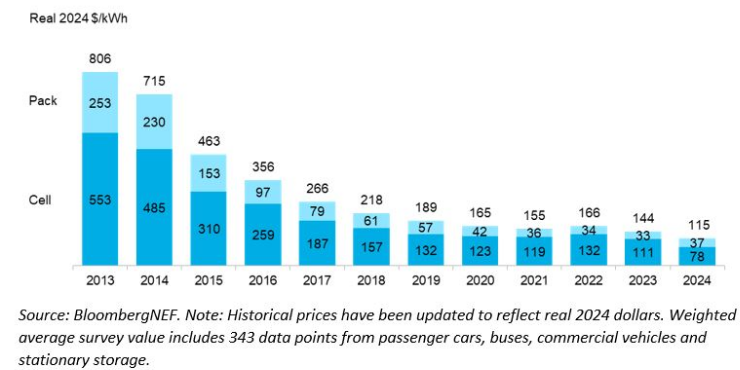
\includegraphics[width=.8\columnwidth]{batVolPrice.png}
                    \caption{Volume-weighted avg. Li-ion Battery Pack and Cell Price Split.}
                    \label{batVolPrice}
                \end{figure}
                The battery capacity, the cost of power, and the total number of charge-discharge cycles are multiplied to get the overall cost of battery charging.
                The sum of the consumer pricing and the battery charging cost is the final definition of the overall cost.

            \subsubsection{Definition of Optimization Criterion}
                The objective function is defined like \cref{fffff}, as the total cost divided by the total driving distance during the vehicle's lifespan, since the purpose is to minimize the cost per range of running a compact EV.
                \begin{align}
                    \label{fffff}
                    f(\vec{x})=\frac{C_{t}(\vec{x})}{R(\vec{x})N}
                \end{align}

                \begin{figure}[h]
                    \centering
                    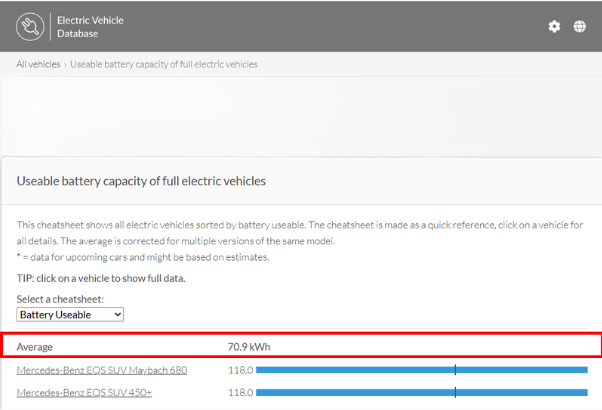
\includegraphics[width=.8\columnwidth]{avgCap.png}
                    \caption{Avg. Battery Capacity of EVs.}
                    \label{avgCap}
                \end{figure}


            \subsubsection{Definition of Constraints}
                \crefrange{eqbegin}{eqend} show the annotated constraints and their explicit expressions.
                \begin{alignat}{3}
                    &g_1: R(\vec{x})&&\geq 400\mathrm{km} && \label{eqbegin} \\
                    &g_2: C_{p} (\vec{x})&&\leq 40\cdot 10^6\text{KRW} &&\\
                    &g_3: \frac{8x_1}{8x_1 +x_2}&&\leq 0.3 &&\\
                    &g_4: x_1 &&\geq 40 &&\\
                    &g_5: x_1 &&\leq 80 &&\\
                    &g_6: x_2 &&\geq 1200 &&\\
                    &g_7: x_2 &&\leq 1800 && \label{eqend}
                \end{alignat}

                Firstly, $g_1$ was chosen since the minimum driving range of the majority of electric cars now available on the market is more than 400 km.
                Then $g_2$ was based on the preference of individuals in their 20s and 30s for EVs that cost less than 40 million KRW \cite{segye24}.
                Furthermore, $g_3$ was established since the existing structural technology cannot handle a battery pack that weighs more than 30\% of the vehicle as a whole.
                Regarding side constraints, the majority of EVs have battery packs that have capacities between 40 and 80 kWh\cite{4080capacity}, which establishes the limits for $x_1$ (See \cref{avgCap}).
                The boundaries for $x_2$ are defined by the fact that the average vehicle weight, excluding the battery pack, falls between 1200 and 1800 kg \cite{glider12}.
            
    \subsection{\textsc{Matlab}}
            This section covers using \textsc{Matlab} to find a minimum solution and verify it graphically.
            \subsubsection{Numerical Solving}
                The following is a sequential description of the code we wrote for the numerical analysis.
                \begin{enumerate}
                    \item First, we initialize the variables, declare the DVs and their side constraints, and define each constant.
                    \begin{lstlisting}
%% init
clearvars;
close all;
clc;

%% dv & bc
% battery capacity; glider weight
DV0=[60;1500]; % initial guess
lb=[40;1200];
ub=[80;1800];

%% params
p=struct();
p.rho=1.2; % density of air
p.g=9.81; % gravity
p.Cd=.35; % drag coefficient
p.Crr=.015; % rolling resistance
p.eta=.9; % efficiency
p.N=1000; % battery charge cycle
p.A=2.2; % frontal pojection area
p.v=12.22; % avg. velocity
p.CE=350; % electricity charge
                    \end{lstlisting}
                    \item Declare anonymous handles.Since the functions we use by default take in both DVs and parameters, we need to wrap them so that they can be optimized with one variable in \texttt{fmincon} (Find minimum of constrained nonlinear multivariable function).
                    \begin{lstlisting}[firstnumber=last]
%% anonymous handles
objFHandle=@(DV)objF(DV(1),DV(2),p);
nonlinConHandle=@(DV)deal(nonlinCon(DV(1),DV(2),p),[]);
                    \end{lstlisting}
                    \item Perform the actual optimization. Here, the algorithm used is \texttt{sqp} (Sequential Quadratic Programming), which has the advantage of convergence stability at small scales. Then print the results to the terminal.
                    \begin{lstlisting}[firstnumber=last]
%% run optimization
opts=optimoptions('fmincon','Algorithm','active-set','Display','none');
[DV_opt,f_opt]=fmincon(objFHandle,DV0,[],[],[],[],lb,ub,nonlinConHandle,opts);

%% print results
fprintf('Design Variables:\nx1=%.3f\tx2=%.f\n\n',DV_opt);
fprintf('Objective Function Value:\nf=%.3f\n\n',f_opt);
fprintf('Analysis Variables:\n');
disp(analyzeVars(DV_opt(1),DV_opt(2),p));
                    \end{lstlisting}
                    \item Define an objective function and nonlinear constraints. The terms in constraints should be transposed so that the expressions are equal to or less than zero. These expressions are returned as a single vector, stacked.
                    \begin{lstlisting}[firstnumber=last]
%% def objective function
function f=objF(cap,wt,p)
    vars=analyzeVars(cap,wt,p);
    f=vars.Ctot./(vars.R*p.N); % cost per range
end

%% def nonlinear constraints
function c=nonlinCon(cap,wt,p)
    vars=analyzeVars(cap,wt,p);
    c=[
        vars.Cprod-40000000; % max cost
        400-vars.R; % min range
        cap-(3/56)*wt % max fraction of battery
        ];
end
                    \end{lstlisting}
                    \item Compute the analysis variables. To keep the processing fast in the \texttt{fmincon} and to allow the grids to be input for later visualization, it is processed using element-wise matrix operations.
                    \begin{lstlisting}[firstnumber=last]
%% def analysis variables
function vars=analyzeVars(cap,wt,p)
    vars=struct();
    vars.E=1/(p.eta*3600).*(p.rho*p.A*p.Cd*p.v^2/2+(8.*cap+wt)*p.g*p.Crr); % energy per distance
    vars.R=cap./vars.E; % range
    vars.Cprod=280000.*cap+6000.*wt+12000000; % production cost
    vars.Cenergy=cap*p.CE*p.N; % energy cost
    vars.Ctot=vars.Cprod+vars.Cenergy; % total cost
end
                    \end{lstlisting}
                \end{enumerate}

            \subsubsection{Graphical Solutions Method}
                \label{gsm}
                The following is a sequential description of the code we wrote for the visualization and graphical solving.
                \begin{enumerate}
                    \item First, we create a mesh grid on the plane and calculate the function value and constraint satisfaction for each point. The calculated range is then divided into equally spaced points on a logarithmic scale, and the satisfactions are all multiplied to form a logical matrix.
                    \begin{lstlisting}
%% construct grids
% visualization area
LB=[30,1050];
UB=[90,1950];

n=1000;
x1=linspace(LB(1),UB(1),n);
x2=linspace(LB(2),UB(2),n);
[X1,X2]=meshgrid(x1,x2);

%% compute functions for plot
f=objF(X1,X2,p);
levels=linspace(log(min(f(:)-50)),log(max(f(:))-50),7);
levels=exp(levels)+50;
levels(2)=f_opt;

c=nonlinCon(X1,X2,p);
% returned as stack of grids
c1=c(1:n,:);
c2=c(n+1:2*n,:);
c3=c(2*n+1:3*n,:);
feasibility=(c1<=0)&(c2<=0)&(c3<=0)&(X1<=ub(1))&(X1>=lb(1))&(X2>=lb(2))&(X2<=ub(2)); % in constraints & boundary
                    \end{lstlisting}
                    \item Prepare a figure, and paint feasible region from the logical matrix. Then draw lines for the constraints in the desired form. Also, draw isocurves using the function intervals recorded and mark the minimum solution at the contact point.
                    \begin{lstlisting}[firstnumber=last]
%% ready figure
figure;
hold on;
box on;

%% draw feasible region
contourf(X1,X2,feasibility,[0.5 1],'LineColor','none','FaceColor','yellow');

%% draw others
% constraints
contour(X1,X2,c1,[0 0],'r--');
text(70,1100,'C_{p}=40M','Color','r','FontWeight','bold');
contour(X1,X2,c2,[0 0],'b--');
text(48,1850,'R=400','Color','b','FontWeight','bold');
contour(X1,X2,c3,[0 0],'g--');
text(78,1600,'56x_1=3x_2','Color','g','FontWeight','bold');

[CF,hF]=contour(X1,X2,f,levels,'LineColor','magenta','LabelFormat','f=%.1f'); % contours
plot([LB(1) UB(1)],[lb(2) lb(2)],'k-'); % boundary
plot([ub(1) ub(1)],[LB(2) UB(2)],'k-');
plot([LB(1) UB(1)],[ub(2) ub(2)],'k-');
plot([lb(1) lb(1)],[LB(2) UB(2)],'k-');
text(50,1175,'x_2=1200','Color','k');
text(80,1500,'x_1=80','Color','k');
text(62,1825,'x_2=1800','Color','k');
text(40,1500,'x_1=40','Color','k');
xlabel('x_1');
ylabel('x_2');
plot(DV_opt(1),DV_opt(2),'o','MarkerSize',10,'MarkerFaceColor','cyan','MarkerEdgeColor','k','LineWidth',2); % solution

clabel(CF, hF, 'FontSize',9, 'Color','m', 'LabelSpacing',400);

%% wrap figure up
axis tight;
xlim([LB(1) UB(1)]);
ylim([LB(2) UB(2)]);
                    \end{lstlisting}
                \end{enumerate}

                \begin{figure}[h]
                    % \begin{minipage}[b]{0.25\textwidth}
                        \centering
                        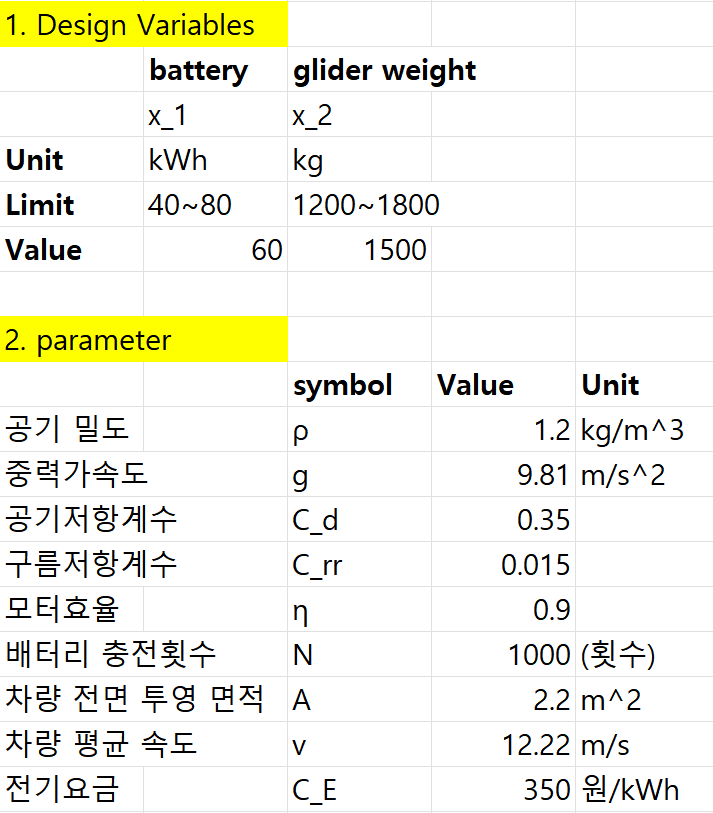
\includegraphics[width=.6\columnwidth]{Excel111.png}
                        \caption{Parameter 1 in Excel.}
                        \label{param1}
                    % \end{minipage}
                    % \hspace{5em}
                \end{figure}

                \begin{figure}[h]
                    % \begin{minipage}[b]{0.45\textwidth}
                        \centering
                        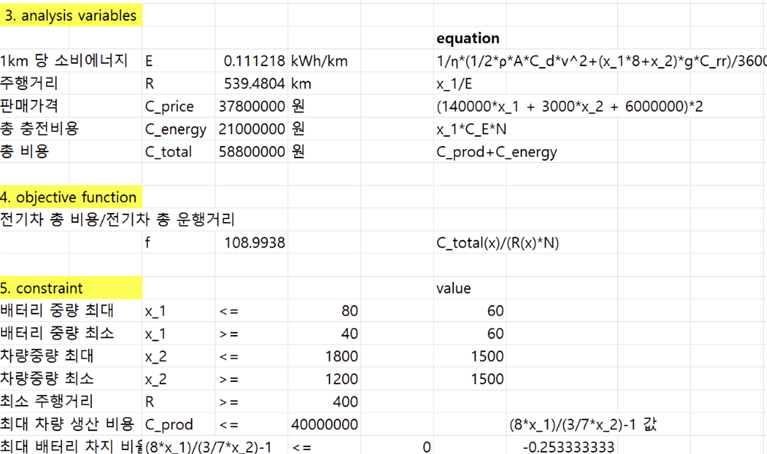
\includegraphics[width=.8\columnwidth]{Excel22.png}
                        \caption{Parameter 2 in Excel.}
                        \label{param2}
                    % \end{minipage}
                \end{figure}
                
        \subsection{Excel}
            \label{methodExcel}
            The following is the process of optimal design using Excel's solver.
            \begin{enumerate}
                \item Organize the DVs, parameters, analysis variables, objective function, and constraints as shown in \cref{param1,param2}, according to the process set in the formalization stage of \cref{form}.
                \item For limiting conditions composed of multiple variables, convert them into a form optimized for Solver application. In our team's design, for example, rewrite the constraint on the maximum ratio of battery weight into the form $\frac{56x_1}{3x_2}-1\leq 0$ for use in Solver.
                \item Turn on the Solver, set the objective function to minimize, enter all constraints including side constraints (a total of 7 in our design), and select the \texttt{GRG} nonlinear solving method. Since the inequality contains a nonlinear equation, this method is appropriate. To minimize errors, use the central difference method for numerical differentiation. Once completed all the settings, it will look like \cref{setting1,setting2}.
                \item After obtaining the results, print the Solver report and sensitivity report to examine the solution and the derivation process.
            \end{enumerate}

            \begin{figure}[h]
                \centering
                % \begin{minipage}[b]{0.40\textwidth}
                    \centering
                    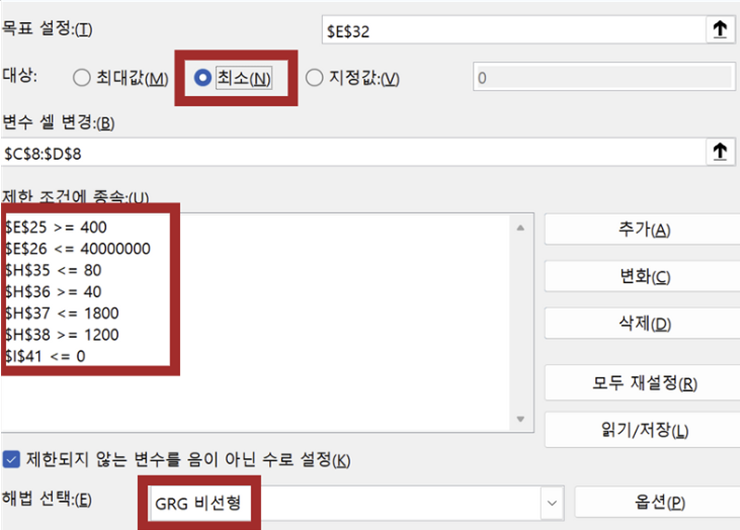
\includegraphics[width=.8\columnwidth]{Excel33.png}
                    \caption{Setting 1 of Solver.}
                    \label{setting1}
                % \end{minipage}
                % \hspace{5em}
            \end{figure}

            \begin{figure}[h]
                % \begin{minipage}[b]{0.40\textwidth}
                    \centering
                    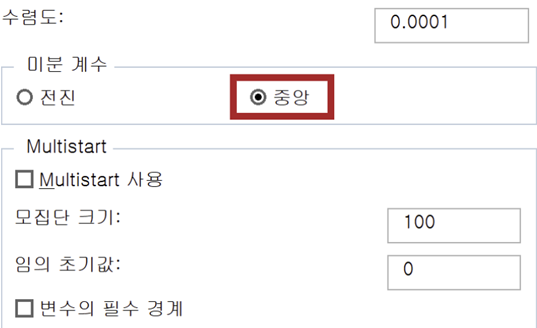
\includegraphics[width=.8\columnwidth]{Excel4.png}
                    \caption{Setting 2 of Solver.}
                    \label{setting2}
                % \end{minipage}
            \end{figure}

        
    \section{Results}
        \subsection{\textsc{Matlab} \texttt{fmincon}}
            The solver converged as shown in \cref{disp}.
            After a total of 11 iterations, the objective function value decreased from 109 to 92.1, while the `norm of step' and the `first-order optimality' showed a repetitive decrease.
            Each index ultimately converged to $7.06\cdot 10^{-8}$ and $4.57\cdot 10^{-8}$, respectively, which were smaller than the set tolerance, so the algorithm terminated.
            \par
            See \cref{disp2}, these are optimum solutions for DVs, objective function value at that point, and calculated analysis variables resulted from solver.
            Looking at the values, we can see that the minimum solution was found at $x_1=64.3$, and at this point, $x_2 = 1200$, which was the boundary of side constraint initially founded.
            In addition, the inequality condition $g_3$, ``the price must be less than 40MKRW,'' was triggered.

            \begin{figure}[h]
                \centering
                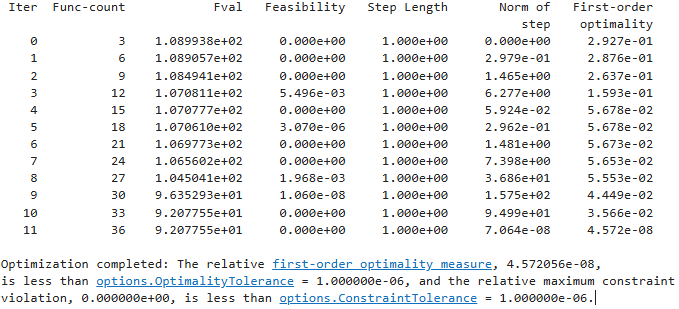
\includegraphics[width=.8\columnwidth]{matlabDisplay.png}
                \caption{Printed Result of Solver.}
                \label{disp}
            \end{figure}

            \begin{figure}[h]
                \centering
                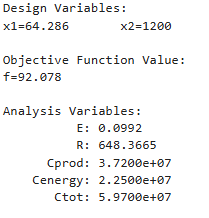
\includegraphics[width=.8\columnwidth]{disp.png}
                \caption{Optimum Solution and Values of Solver.}
                \label{disp2}
            \end{figure}

        \subsection{Visualization}
            \label{vis}
                \cref{graphical} illustrates the result figure of code discussed in \cref{gsm}.
                First, the areas surrounded by black solid lines and restricted by RGB dashed lines are considered as the feasible region in yellow.
                Next, examining the magenta contour lines, we observe that the function values decrease as you move toward the bottom-right, converging to the optimal point.
                Eventually, the optimal solution can be found at the point where the last contour line is about to leave-the intervals were intentionally set so that the line passes through the point-the feasible area.

                \begin{figure}[h]
                    \centering
                    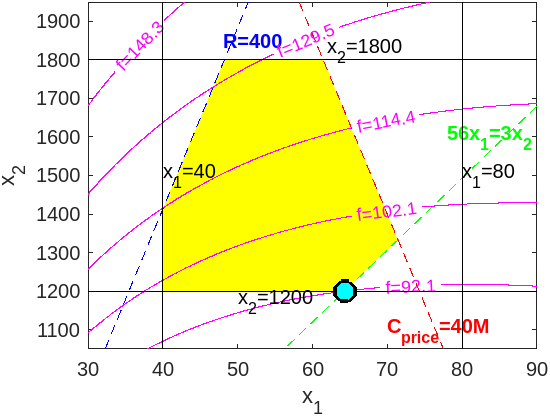
\includegraphics[width=.9\columnwidth]{graphical.png}
                    \caption{Graphical Solutions.}
                    \label{graphical}
                \end{figure}

        \subsection{Excel}
            Solver's results were derived as in \cref{res1,res2}.
            Similar to the optimal solution using \textsc{Matlab}, the battery capacity was about 64.28 kWh, the weight of the body excluding the battery was 1,200kg, and the objective function, that is, the vehicle cost per range, was about 92.08 won.

            \begin{figure}[h]
                % \centering
                % \begin{minipage}[b]{0.25\textwidth}
                    \centering
                    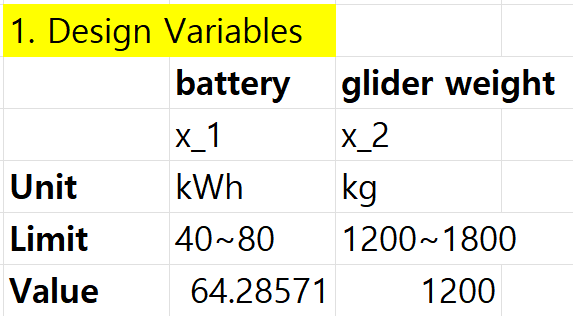
\includegraphics[width=.8\columnwidth]{Excel55.png}
                    \caption{Results of design variables.}
                    \label{res1}
            \end{figure}

            \begin{figure}[h]
                % \end{minipage}
                % \hspace{5em}
                % \begin{minipage}[b]{0.40\textwidth}
                    \centering
                    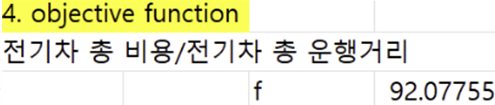
\includegraphics[width=.8\columnwidth]{Excel6.png}
                    \caption{Result of objective function.}
                    \label{res2}
                % \end{minipage}
            \end{figure}

            \par
            As mentioned in the \cref{methodExcel}, the sensitivity of the variable can be confirmed by obtaining the Lagrange multiplier value of each constraint through the sensitivity report.
            \cref{sense1} is a sensitivity report of the optimal design.
            As can be seen here, it can be seen that the absolute value of the Lagrange multiplier of the maximum charge ratio of the battery weight is about 7.9, which is significantly higher than that of other constraints.
            
            \begin{figure}[h]
                \centering
                % \begin{minipage}[b]{0.40\textwidth}
                    \centering
                    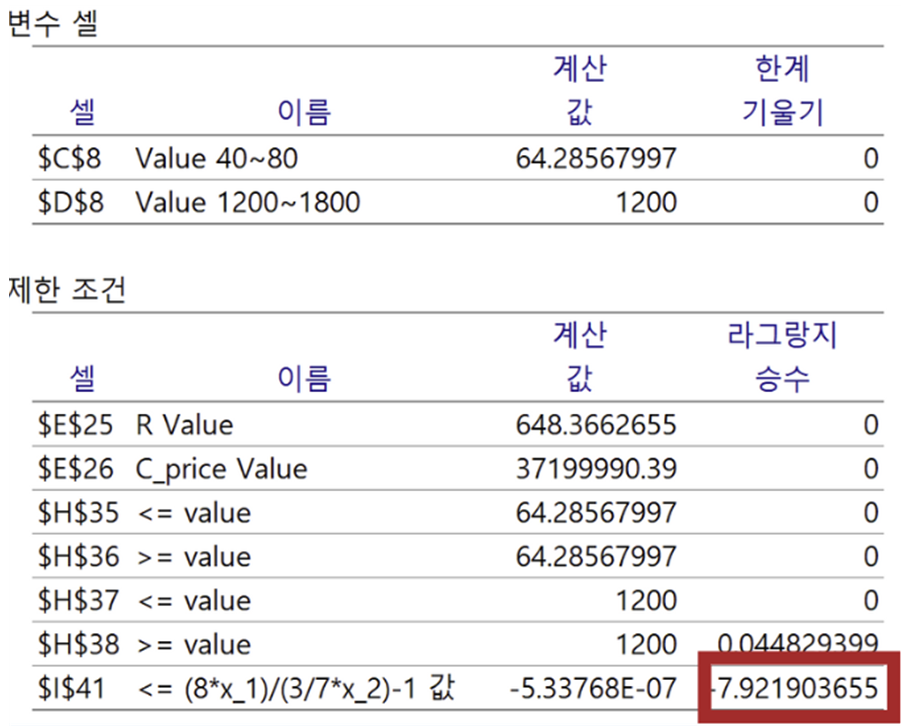
\includegraphics[width=.8\columnwidth]{Excel77.png}
                    \caption{Sensitivity report of Solver.}
                    \label{sense1}
                % \end{minipage}
                % \hspace{5em}
            \end{figure}

            \begin{figure}[h]
                % \begin{minipage}[b]{0.40\textwidth}
                    \centering
                    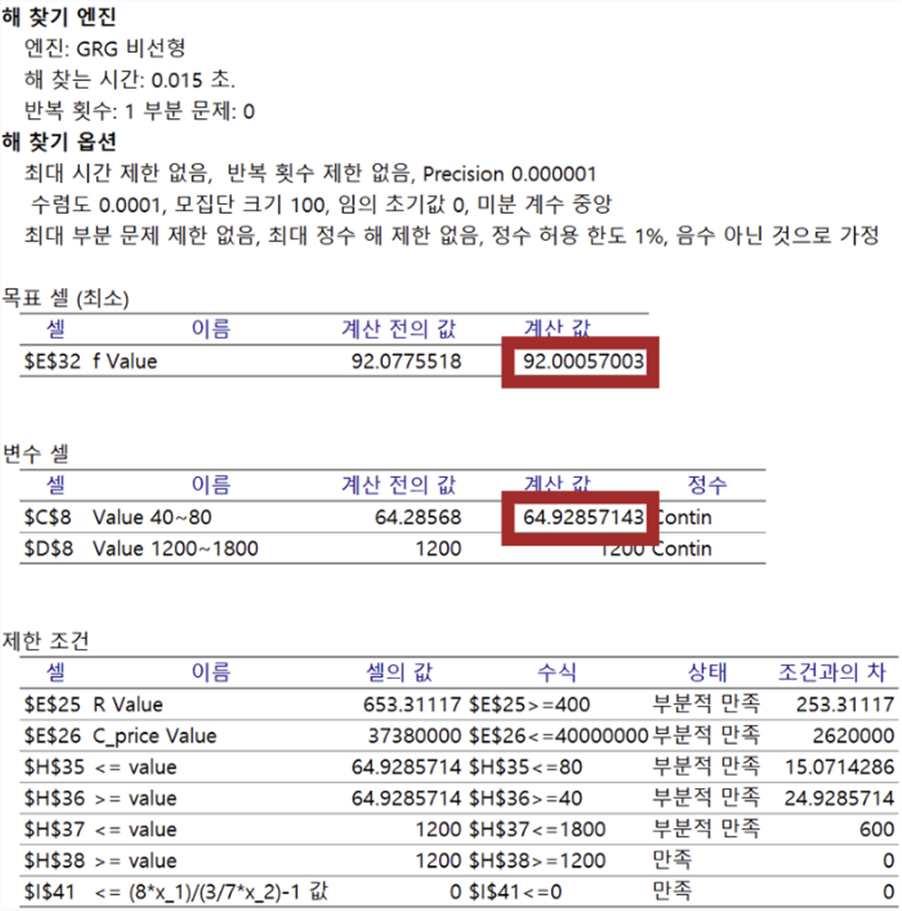
\includegraphics[width=.8\columnwidth]{Excel88.png}
                    \caption{New result with offset.}
                    \label{sense2}
                % \end{minipage}
            \end{figure}

            Therefore, if the maximum charge ratio of the battery weight is relaxed, it can be expected that a more ideal value can be obtained.
            \cref{sense2} is the result derived by giving an offset of 1 percent above.
            In the objective function, a decrease of about 0.08 won and an increase of about 0.7 kWh in the battery capacity.
            Finally, an ideal value suitable for the purpose was obtained.


    \section{Discussion}
        \subsection{Insights from Graphical Solutions}
            In general, solvers such as \texttt{fmincon} cannot guarantee that the solution they find is the global minimum.
            Therefore, it is important to check whether the optimization process may have settled on a local minimum, which could lead to misinterpretation.
            Looking at \cref{graphical}, the contour lines do not form a closed curve within the feasible region.
            Instead, they appear to decrease monotonically toward the bottom-right corner.
            This suggests that the function value keeps decreasing in that direction, and the point found is likely the actual minimum.
            \par
            As discussed in the \cref{vis}, a solution is typically found where a contour line of the objective function touches the boundary of the feasible region.
            At this intersection, the slope of the contour line lies between the slopes of the active constraints — in other words, the tangent of the objective function aligns with the constraints at a single point.
            This geometric situation strongly supports the uniqueness of the solution, since it is the only point where both the optimality condition of the objective and the constraint activation are satisfied.
            Therefore, within the search range, the solution is likely unique.
            \par
            These two paragraphs support the absence of a local minimum and the uniqueness of the solution.
            If a more rigorous mathematical justification is needed, we can refer to the Hessian matrix and the KKT conditions.
            If, over the domain, the Hessian is not stationary and remains positive (semi-)definite, this indicates no other local minimum exists.
            Moreover, if the gradient of the Lagrangian is zero and the Lagrange multipliers are positive near the solution, this further confirms uniqueness.
            Unfortunately, we were not able to verify these conditions directly in \textsc{Matlab} code.

        \subsection{Excel}
            Excel's Solver offered a convenient way to handle our nonlinear optimization with multiple constraints.
            Its simple interface allowed us to test DVs and constraints quickly without writing code, making it effective for early-stage analysis.
            \par
            However, Solver is sensitive to initial values and may converge to a local, not global, optimum.
            Complex constraints also require reformulation to fit Solver's format, which can limit flexibility.
            \par
            Overall, Solver is best used for low-complexity problems or preliminary exploration.
            For more advanced optimization, pairing it with tools like \textsc{Matlab} can improve reliability and control.

        \subsection{The Optimal Solution Reaching the Boundary of the Side Constraint: Vehicle Weight Excluding the Battery}
            Based on various assumptions and simulation methods, we concluded that a battery capacity of approximately 64.28 kWh and a vehicle body weight excluding the battery of about 1200 kg was the most ideal combination.
            This value defines the relationship between cost, performance, and weight, and was considered the optimal setting under the given conditions.
            \par
            One particularly noteworthy aspect during the analysis was that the vehicle weight excluding the battery was calculated as the boundary value of the side constraint throughout the entire process.
            In the current electric vehicle manufacturing process, one of the most difficult issues is the relationship between battery capacity and weight.
            With current technology, battery weight cannot increase unless the total vehicle weight increases.
            However, since there is a physical limitation on how much weight the battery can occupy, if the vehicle body weight does not exceed a certain level, it becomes difficult to increase the battery size, and eventually there is no choice but to accept a loss in driving distance.
            \par
            Nevertheless, through this optimal design, we were able to directly realize why the vehicle weight should be kept low in terms of both cost and performance.
            In future vehicle development, a comprehensive approach including structural design, material selection, and battery technology will be necessary, and we believe this is a challenge that must be solved in the automobile industry in the near future.
        \subsection{Limitations}
            Meanwhile, this design was carried out under the assumption of ideal usage conditions, where full charge/discharge cycles are repeated.
            However, in actual battery use, full charge and full discharge can be critically harmful to battery performance.
            For this reason, such a pattern is not common, and charging cycles can vary depending on user driving habits, charging infrastructure, seasonal factors, and other variables.
            In addition, the rising electricity fees and vehicle maintenance costs over time were excluded from this model (See \cref{bill}), and these can act as potential sources of error affecting the accuracy of the result.
            \par
            If future research reflects these factors more precisely, a more realistic and reliable optimal design can be expected.
            Through this project, we experienced firsthand that optimal design is not just about numerical calculation, but a meaningful tool for solving real engineering problems.

            \begin{figure}[h]
                \centering
                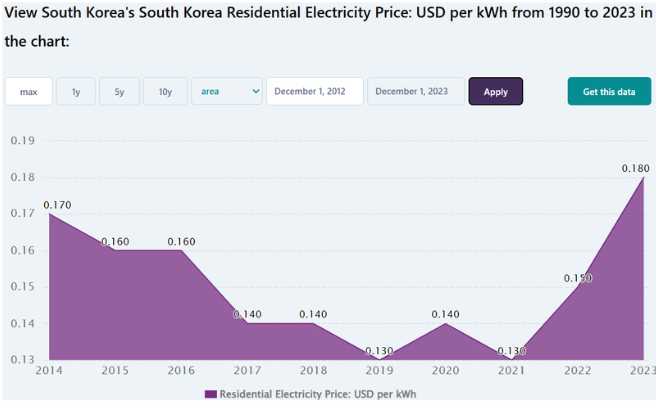
\includegraphics[width=0.8\columnwidth]{bill.png}
                \caption{Increasing Electricity Bill.}
                \label{bill}
            \end{figure}
            
    \printbibliography
\end{document}
